\subsection{design}
Til forstærkningen er der brugt en ikke-inverterende forstærker. Ved en ikke-inverterende forstærker bliver inputtet tilkoblet direkte til den ikke-inverterende inputterminal. Dette er gjort for operations forstærkeres inputimpedans kan udnyttes\fxnote{Evt. skrive TI81’s impedans som er 10^12, og sæt datablad som kilde}. Derudover bliver signaler ikke inventeret ved forstærkningen, hvilket betyder at inputtet og outputtet har samme polaritet. Kredsløbet består af et closed-loop med modstandene R$1$ og R$2$, som udgør en spændingsdeler, som det ses på \figref{Forstaerker}.
\begin{figure}[H]
\centering
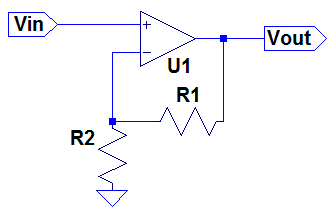
\includegraphics[scale=1]{figures/cProblemloesning/Forstaerker.PNG}
\caption{Kredsløbet for en ikke-inverterende forstærker i en closed-loop konfiguration.}
\label{fig:Forstaerker}
\end{figure} 

Der er jævnført \ref{OpsamlingsAfs} bestemt at forstærkningen skal være en faktor $18$, hvilket svarer til $25.1055$dB. For at udregne modstandene er R$2$ blevet fastsat til $10$K\Omega og ud fra dette er R1 blevet bestemt ved følgende udregning:
\begin{equation} \label{eq:Forstaeker_faktor18}
18=1+\left ( \frac{R1}{10K\Omega } \right )\\
R1 = 170K\Omega
\end{equation}

Disse modstande er blevet brugt til at designe kredsløbet for en ikke-inverterende operations forstærker. Dette kredsløb er designet i LT-spice, som ses på \figref{Forstaerker_faktor18}. 
\begin{figure}[H]
\centering
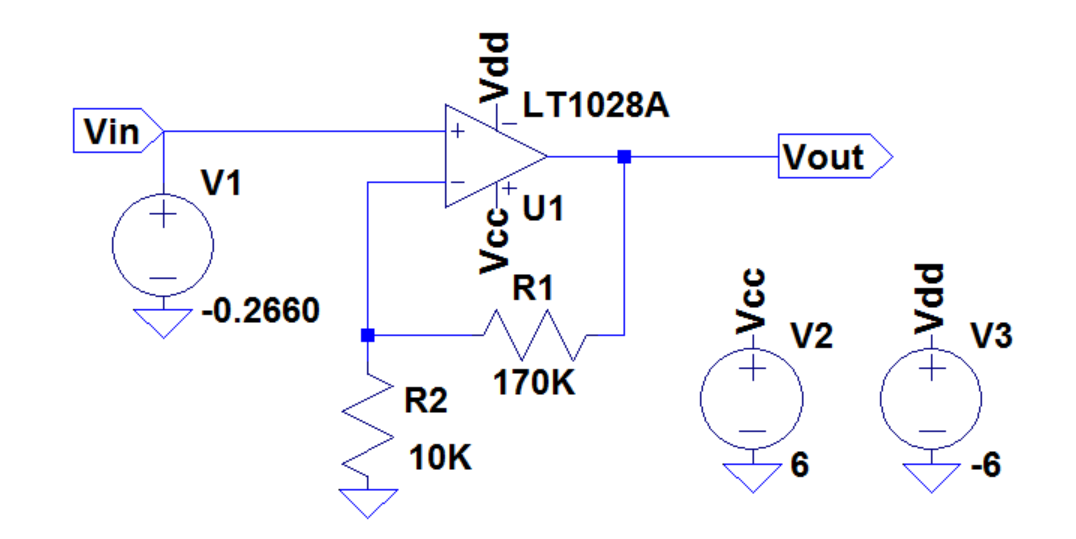
\includegraphics[scale=1]{figures/cProblemloesning/Forstaerker_faktor18.PNG}
\caption{Kredsløbet for en ikke-inverterende forstærker med to modstande, R$1$ og R$2$, som med værdierne $10$K\Omega og $170$K\Omaga giver en forstærkning med en faktor 18.}
\label{fig:Forstaerker_faktor18}
\end{figure} 

Det kan ses på \figref{Forstaerker_faktor18_simulering}, at det forstærkede signal, kaldet Vout er $1.8$V, hvilket er $18$ gange større end Vin, som i simuleringen er sat til $0.1$V. Derved er der sket den ønskede forstærkning, hvilket var forventet, da simuleringen er med ideelle komponenter, og derfor har de enkelte komponenter ingen tolerance, som der vil være ved reelle komponenter i et reelt kredsløb. 

\begin{figure}[H]
\centering
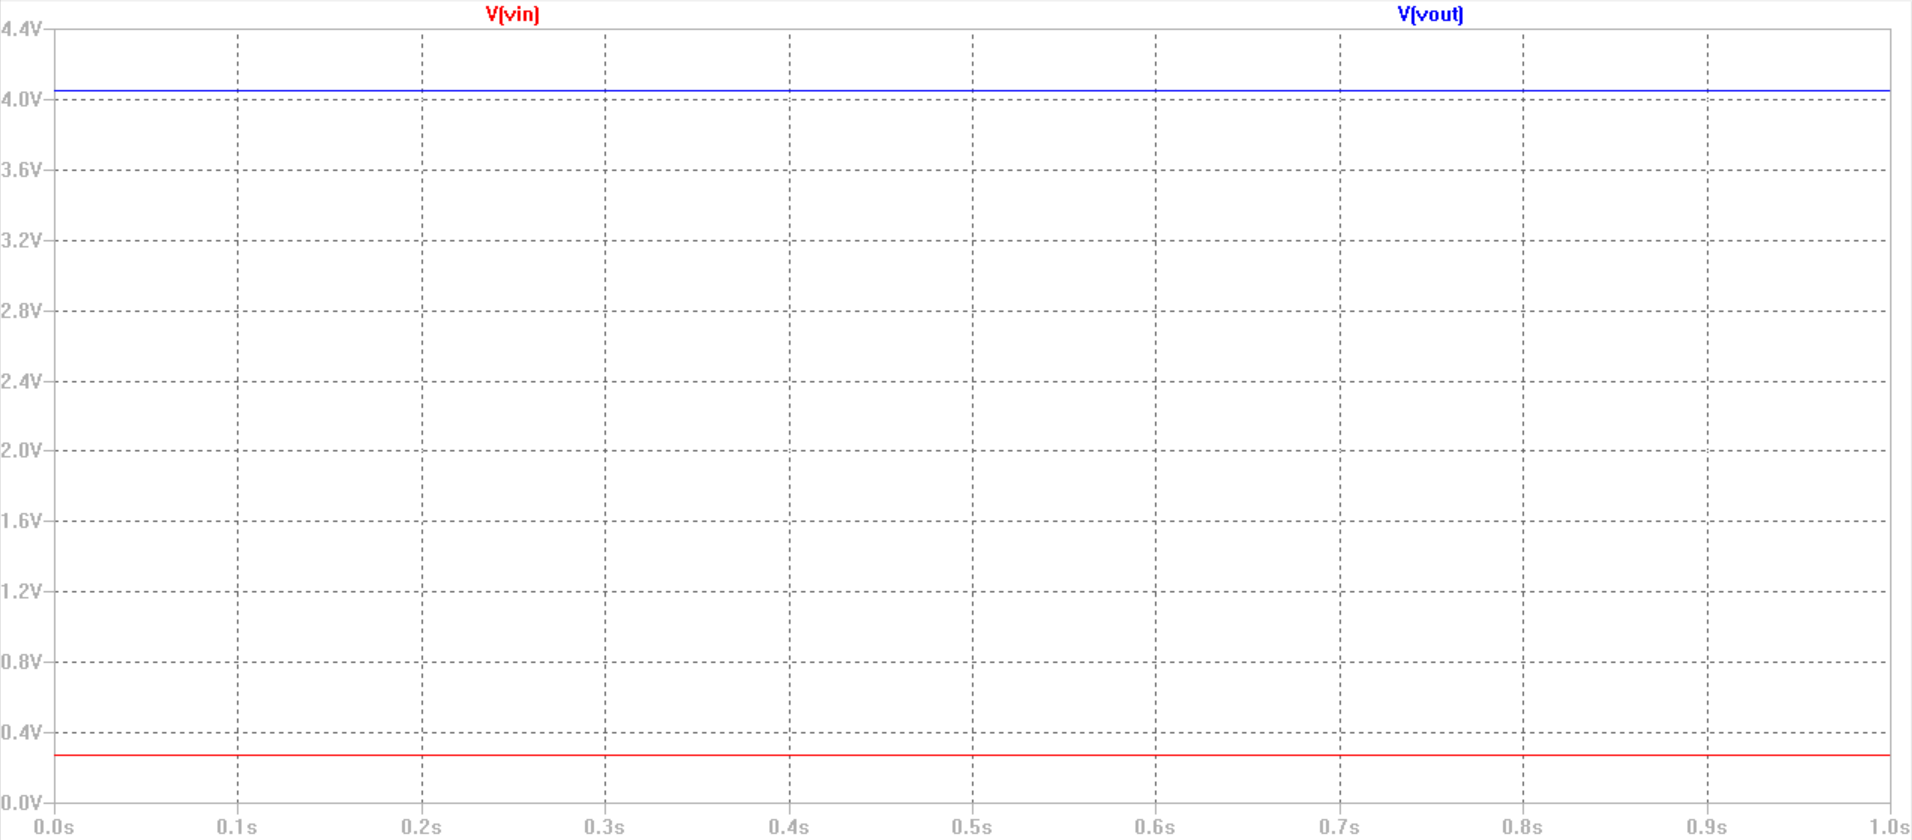
\includegraphics[scale=1]{figures/cProblemloesning/Forstaerker_faktor18_simulering.PNG}
\caption{En simuleringen af en ikke-inverterende forstærker som set på \figref{Forstaerker_faktor18}, hvor der er en forstærkning med en faktor 18. Dette kan på figuren ses at inputtet, Vin, er 0.1V, som bliver forstærket 18 gange, så outputtet, Vout, er 1.8V}
\label{fig:Forstaerker_faktor18_simulering}
\end{figure} 